\documentclass[../report]{subfiles}
\setcounter{section}{0}
\begin{document}

本章では,本プロジェクトの背景と目的を説明する.

\section{認知症の現状} \label{sec:genzyou}
近年の日本国内では,認知症患者数が増加傾向にある.
二宮によると,2012年時点で日本国内の推定認知症患者数は462万人であったが,2025年では675万人,2040年では802万人に上るとしている(図\ref{fig:nintisyo-graph}).
また同研究によると,65歳以上の高齢者の推定認知症有病率は2012年では15.5%,2025年では20.6%,2040年では25.4%と,年々増加する傾向にあるとされている.
また,認知症の発症には生活習慣,特に食習慣や運動習慣,睡眠習慣が関わっていることが分かっている\cite{seikatsu}.
\begin{figure}[htbp]
    \begin{center}
        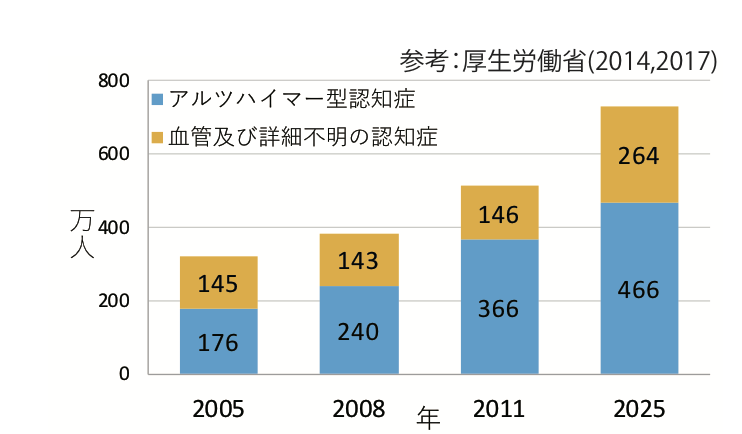
\includegraphics[width=10cm]{imgs/ninchisyo-graph.png}
        \caption{日本の認知症の総患者数の推移}
        \label{fig:ninchisyo-graph}
    \end{center}
\end{figure}
\bunseki{佐藤碧}

\section{現状における問題点} \label{sec:mondai}
日本では高齢化が進んでおりまたその傾向が今後も続いていく中で,介護者不足が問題となっており,もはや高齢者は単なる庇護対象でいるだけでは不十分である.
むしろ積極的に自身の健康管理に関わっていき,病気の予防に努めるべきである.
その中で,認知症予防のためには\ref{sec:genzyou}でも上げたように自身の生活習慣を知り,問題があれば改善することが重要である.
そのための手段としてはライフログの記録・可視化といったことが挙げられる\cite{lifelog}.
そのための手段としては,一般にはICTが用いられている.
ICTを利用する利点としては,蓄積した情報を管理・解析するのが容易であるということが挙げられるが.一方で,高齢者の方にはICTに苦手意識があったり,そもそも利用したことがないといったことがある.
このように,高齢者のICTを利用したライフログ取得・管理には問題がある.
また,医療従事者が認知症医療での医療選択をする際の判断材料が不足しているといった問題もある.
従来の医療従事者が知り得た患者に関する情報は,診察から得られるその時点での情報に限定されていた.
むしろ治療には,どのような過程で今のような状態に至ったのかといったような長期的な情報が必要である.
だが現状では,それらを実現するような仕組みは整備されていないという現状がある.
\bunseki{佐藤碧}

\section{目的}
\ref{sec:mondai}で挙げた問題点を解決するために本グループでは,ライフログの可視化による生活習慣の改善,ICTに不慣れな人でも容易にライフログを取得できる手段の開発,医療選択時に必要となる情報の蓄積といったことを目指す.
\bunseki{佐藤碧}

\end{document}
